\documentclass[11pt,a4paper]{article}
\usepackage[margin=15mm]{geometry}\usepackage{fontspec,amsmath,graphicx,booktabs}
\setmainfont{Latin Modern Roman}\setlength{\parindent}{0pt}\setlength{\parskip}{7pt}
\begin{document}
{\Large Alternative stationary-field solution: inspect before constraints}

Same shared-field model, uniform final-arc references and fixed correspondence. Existing saved solution (run 10); no new fit or constraints. Top: previously selected minimum-cost solution. Bottom: alternative local solution. All curves below are in signal space.

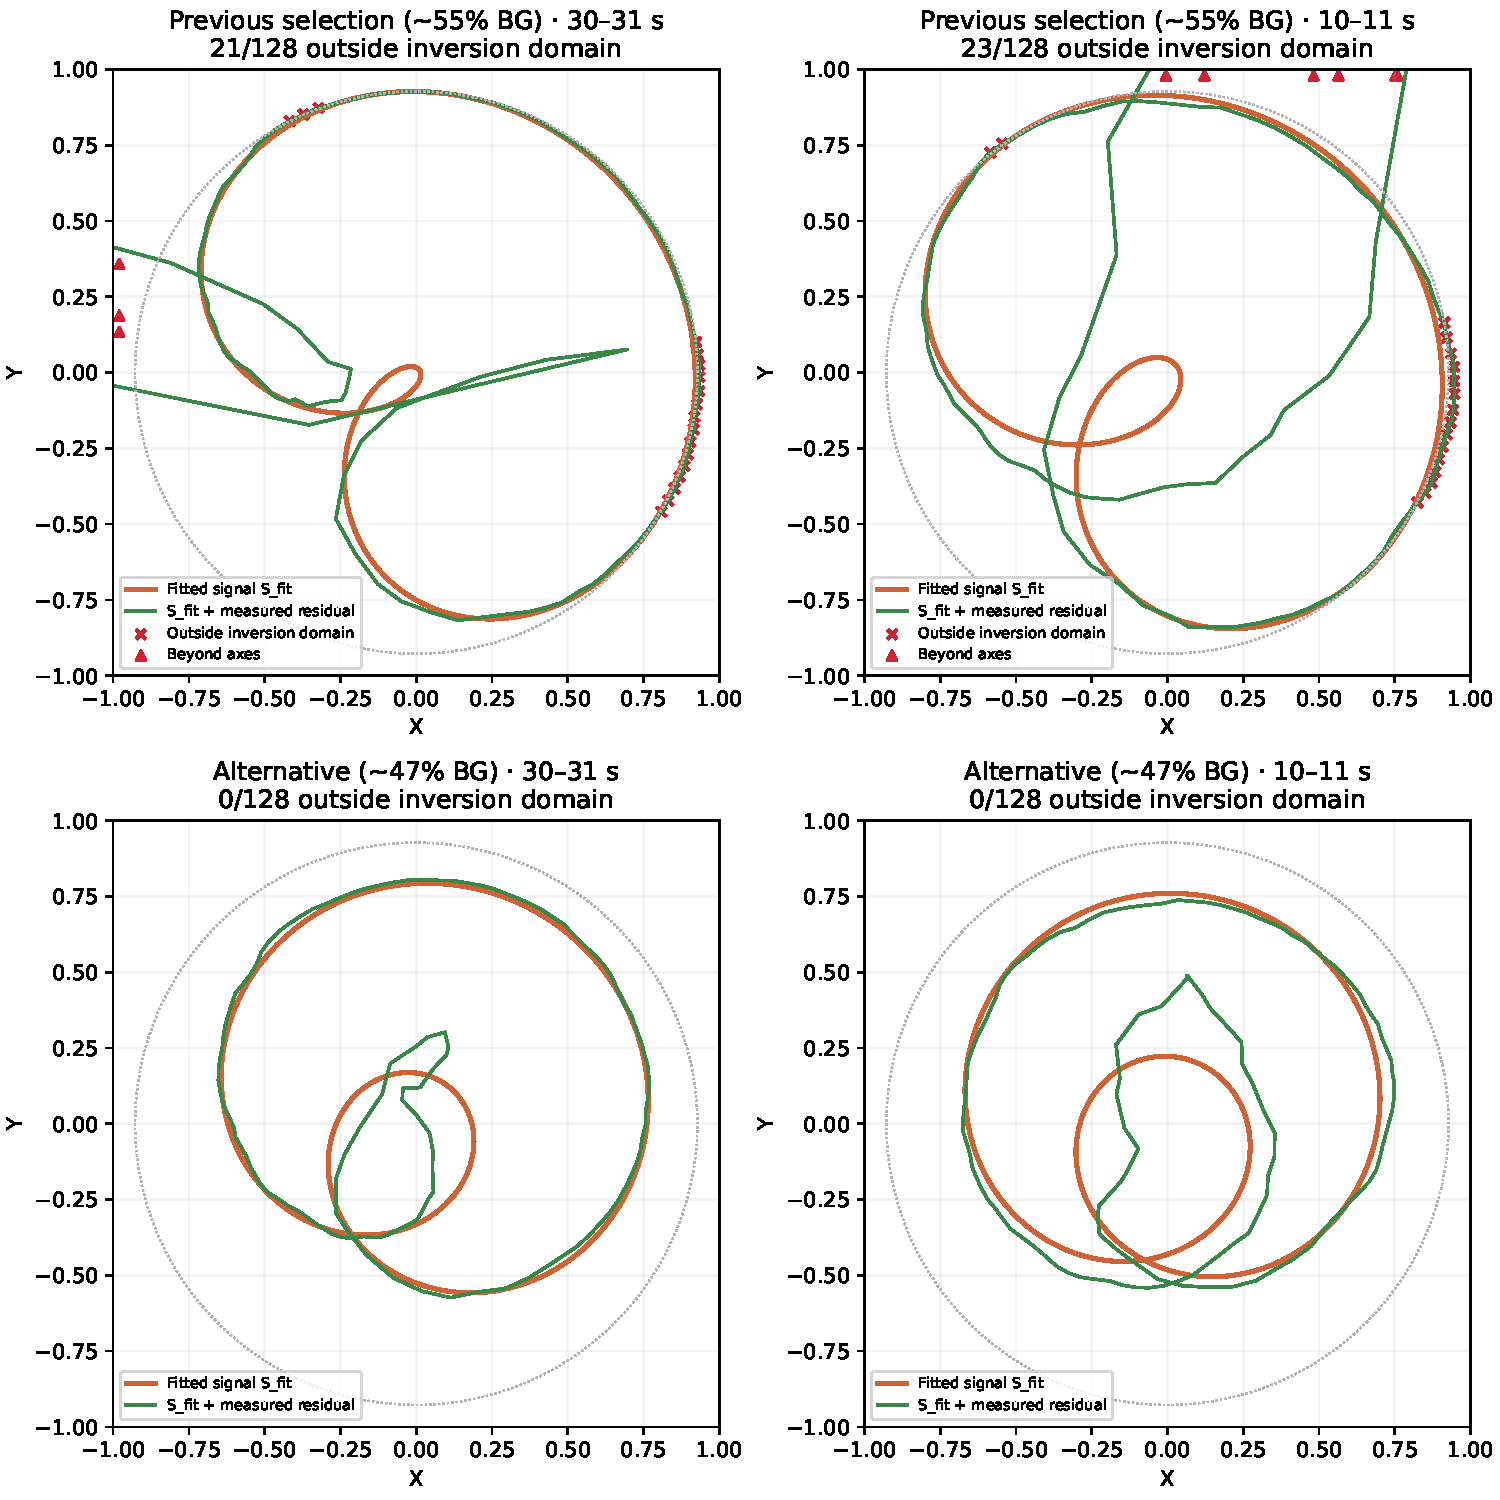
\includegraphics[width=\linewidth]{comparison.pdf}

The alternative has no invalid corrected held-out points in either window. The remaining differences are visible; this is improved recovery behaviour, not verified absolute angles. Red boundary triangles locate off-axis points schematically; no corrected points have been physically clipped.
\newpage
{\Large Alternative: measured-space fit and signal-space recovery}

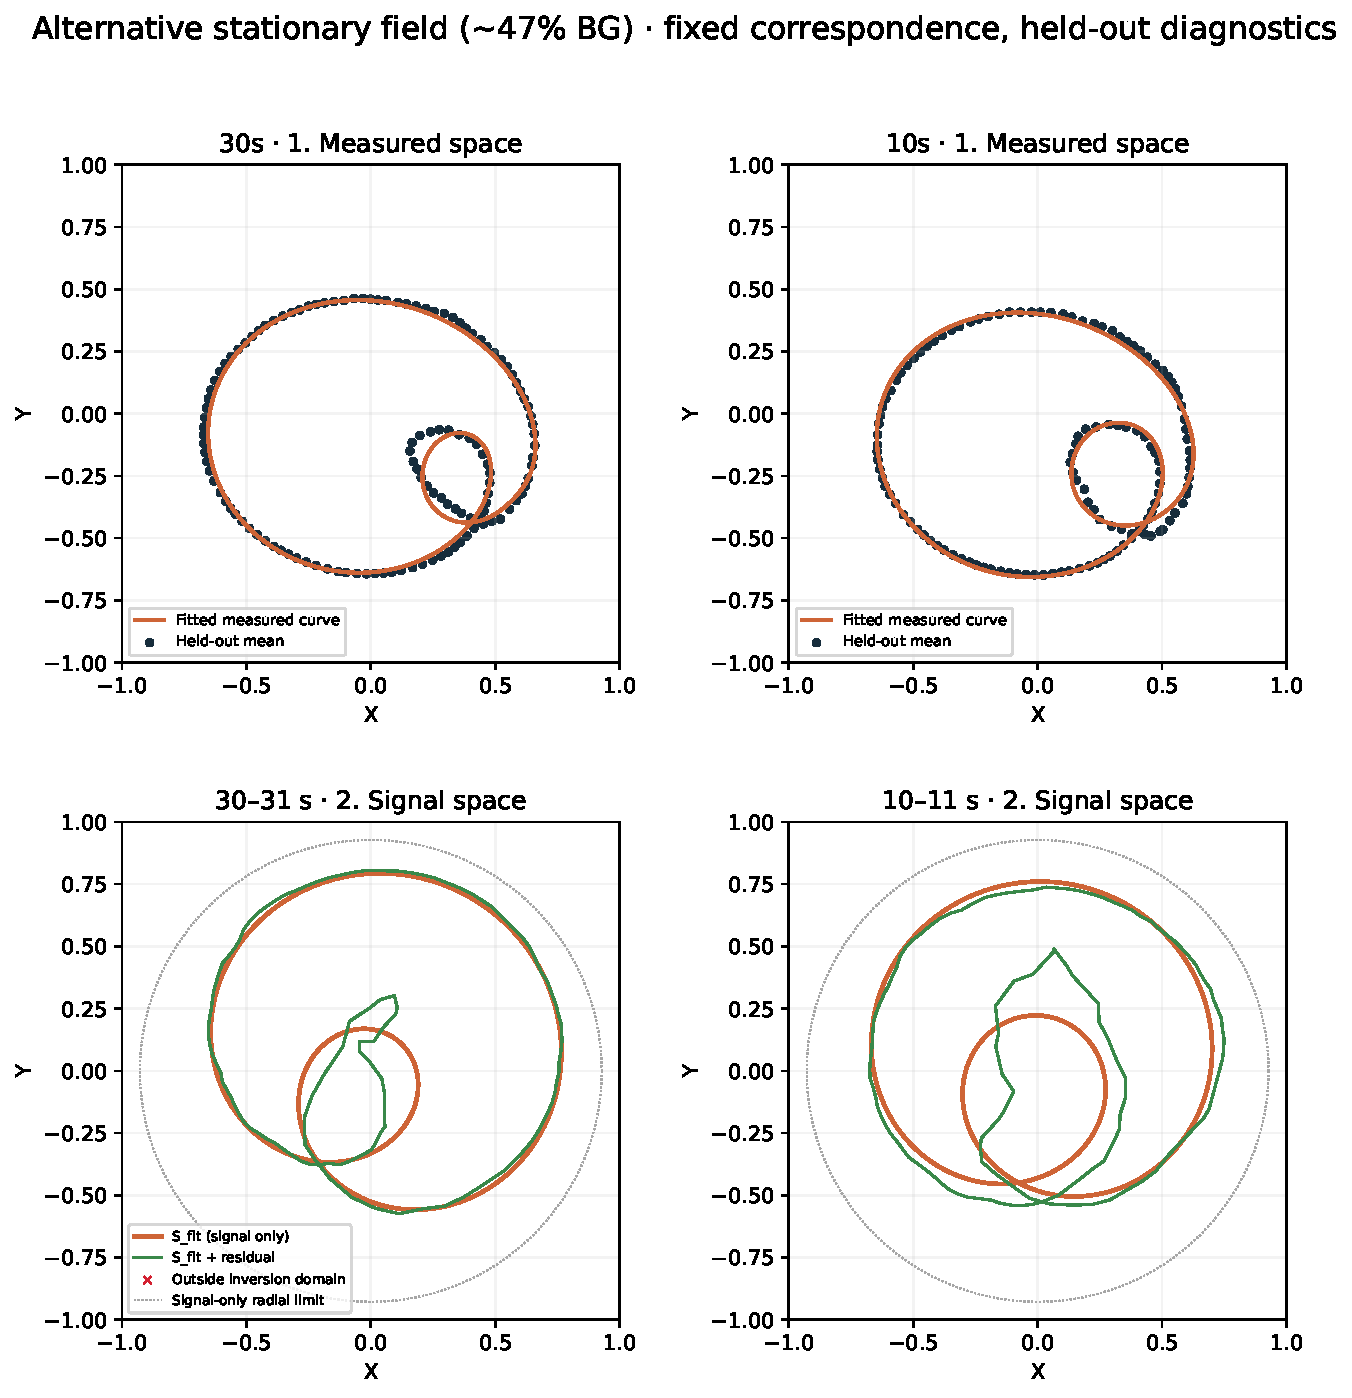
\includegraphics[width=\linewidth]{stationary.pdf}

The same fixed background field is shared across both windows. Background is 47.59\% / 47.33\% of the respective original maximum total intensity. Correction is conditional: interference is evaluated at the matched fitted orientation before subtraction. The field has not been re-estimated at each reconstructed direction.
\newpage
{\Large Alternative: laboratory sphere and cone-frame residuals}

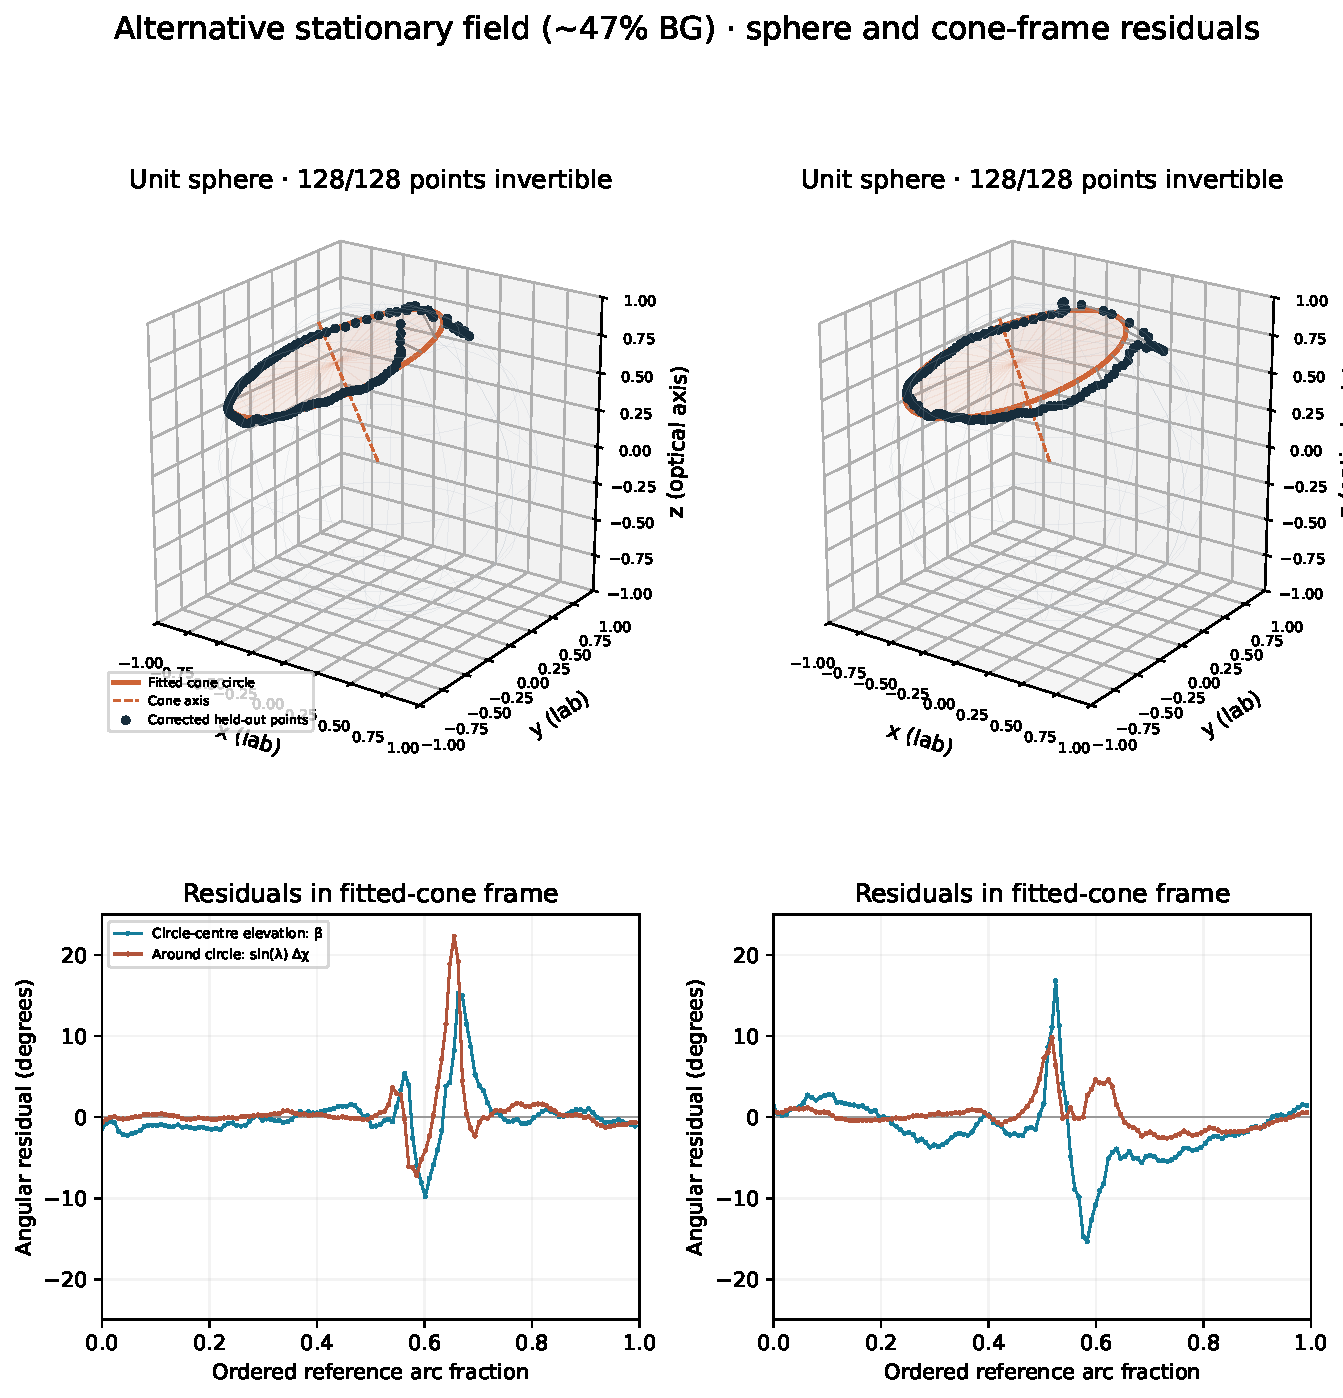
\includegraphics[width=\linewidth]{stationary_sphere.pdf}

Sphere points are corrected held-out observations, with each measurement-degenerate branch chosen nearest its matched fitted cone point. Blue residual is circle-centre elevation $\beta$; orange is $\sin\lambda\,\Delta\chi$. The residual axes are set to $\pm25^\circ$ to show the remaining structure.
\newpage
{\Large Numerical comparison and interpretation}

\begin{tabular}{llrrr}\toprule
Window & Solution & Measured RMS & Signal RMS & Invalid/128\\\midrule
30--31 s & Previous & .00506 & .0488 & 21\\
30--31 s & Alternative & .00570 & .0120 & 0\\
10--11 s & Previous & .00954 & .0575 & 23\\
10--11 s & Alternative & .00991 & .0182 & 0\\\bottomrule\end{tabular}

Measured RMS divides each channel error by measured total intensity at that point; signal RMS divides it by fitted total rod signal. These are four-channel RMS values, not anisotropy distances or single-channel percentage errors.

\begin{tabular}{lrr}\toprule
Alternative, all 128 points & 30--31 s & 10--11 s\\\midrule
Circle-centre elevation RMS & $3.17^\circ$ & $4.45^\circ$\\
Around-circle displacement RMS & $3.64^\circ$ & $2.08^\circ$\\
Geodesic angular RMS & $4.57^\circ$ & $5.02^\circ$\\
Corrected pair-imbalance RMS & 0.52\% & 0.54\%\\\bottomrule\end{tabular}

Geodesic RMS is the angle between the corrected, branch-selected direction and its matched fitted direction. It is not an error against known rod angles. The previous solution's valid-only angular scores exclude its failed inversions and cannot be directly compared as if they covered the same samples.

The alternative has a slightly worse measured-intensity objective but much better subtraction behaviour. The old objective alone preferred the solution with more severe signal-space distortion. No new constraints have yet been imposed. Selection by inspecting held-out diagnostics is exploratory; a subsequent constrained fit needs training-side selection and fresh validation data before claiming independent validation.

All optics, calibration, fitted correspondence and data averaging are unchanged. These are existing local solutions, not globally certified optima. No commit or push.
\end{document}
